\documentclass[12pt]{article}
\usepackage[utf8]{inputenc}
\usepackage[dvips]{graphicx}
\usepackage{epsfig}
\usepackage{fancybox}
\usepackage{verbatim}
\usepackage{array}
\usepackage{latexsym}
\usepackage{alltt}
\usepackage{amssymb}
\usepackage{amsmath}
\usepackage{hyperref}
\usepackage{listings}
\usepackage{color}
\usepackage{algorithm}
\usepackage{algpseudocode}
\usepackage[hmargin=3cm,vmargin=5.0cm]{geometry}
\usepackage{epstopdf}

\usepackage[section]{placeins}
\usepackage{caption}
\usepackage{subcaption}

\topmargin=-1.8cm
\addtolength{\textheight}{6.5cm}
\addtolength{\textwidth}{2.0cm}
\setlength{\oddsidemargin}{0.0cm}
\setlength{\evensidemargin}{0.0cm}
\newcommand{\HRule}{\rule{\linewidth}{1mm}}
\newcommand{\kutu}[2]{\framebox[#1mm]{\rule[-2mm]{0mm}{#2mm}}}
\newcommand{\gap}{ \\[1mm] }
\newcommand{\Q}{\raisebox{1.7pt}{$\scriptstyle\bigcirc$}}
\newcommand{\minus}{\scalebox{0.35}[1.0]{$-$}}



\lstset{
    %backgroundcolor=\color{lbcolor},
    tabsize=2,
    language=MATLAB,
    basicstyle=\footnotesize,
    numberstyle=\footnotesize,
    aboveskip={0.0\baselineskip},
    belowskip={0.0\baselineskip},
    columns=fixed,
    showstringspaces=false,
    breaklines=true,
    prebreak=\raisebox{0ex}[0ex][0ex]{\ensuremath{\hookleftarrow}},
    %frame=single,
    showtabs=false,
    showspaces=false,
    showstringspaces=false,
    identifierstyle=\ttfamily,
    keywordstyle=\color[rgb]{0,0,1},
    commentstyle=\color[rgb]{0.133,0.545,0.133},
    stringstyle=\color[rgb]{0.627,0.126,0.941},
}


\begin{document}

\noindent
\HRule %\\[3mm]
\small
\begin{center}
	\LARGE \textbf{CENG 483} \\[4mm]
	\Large Introduction to Computer Vision \\[4mm]
	\normalsize Fall 2021-2022 \\
	\Large Take Home Exam 3 \\
	\Large Image Colorization \\
    \Large Student ID: 2375574 \\
\end{center}
\HRule

\begin{center}
\end{center}
\vspace{-10mm}
\noindent\\ \\ 
Please fill in the sections below only with the requested information. If you have additional things to mention, you can use the last section. Please note that all of the results in this report should be given for the \textbf{validation set} by default, unless otherwise specified. Also, when you are expected to comment on the effect of a parameter, please make sure to \textbf{fix} other parameters. You may support your comments with visuals (i.e. loss plot).

\section{Baseline Architecture (30 pts)}
    Based on your qualitative results (do not forget to give them),
    \begin{itemize}
        \item Discuss effect of the number of conv layers:
        \item Discuss effect of the kernel size(except the last conv layer):
        \item Discuss effect of the number of kernels(except the last conv layer):
        \item Discuss effect of the learning rate by choosing three values: a very large one, a very small one and a value of your choice:

    \end{itemize}

    \vspace*{0.5cm}
    \begin{center}
        \raggedright
        As number of convolutional layers increases, the network capacity increases. Hence, model can fit to data more strictly.
        Learning the model with 4-convolution requires more time, since capacity is much greater than 2-conv and 1-conv networks and we can observe this phenomenon in Figure-\ref*{fig:conv_layers}
        where red curve decreases slower than green and orange curves. One interesting observation is that why 4-conv has more train-loss than lower capacity networks, since theoretically it has more capacity
        to overfit/memorize the train-data, the reason is that probably we haven't gave him enough epochs to memorize the train-data since max-epochs is restricted to be 100. 
        However, my observation is that after 20-40 epochs, rate of change of 4-conv is greater than 2-conv and 1-conv meaning that 
        it keeps decreasing more even if it's slow. Another interesting observation is that why train-loss and valid-losses are almost the same at every epoch, the reason is that
        problem is not very difficult, we are trying to colorize the facial images and also train data and valid data are very similar and balanced.
        So it's expected to get similar curves for both valid-loss and train-loss.
        \\
        Common Hyperparameter Baseline in Exp: \\
        learning-rate = 0.001, batch-size = 16, epoch = 100, kernel-num=8, kernel-size=3
        \\~\\

        I've experimented with different kernel sizes of 3 and 5 for both 2-conv and 4-conv networks.
        For both of these models 5x5 kernel yields better performance than 3x3 kernel as illustrated in Figure-\ref*{fig:conv_kernels}.
        Higher spatiality with larger kernels for convolution improves performance in this task. 
        The optimal kernel size depends on the problem and the configuration, however in this problem higher spatiality over kernels allows us to get better estimations
        for the face pixels.
        \\
        Common Hyperparameter Baseline in Exp: \\
        learning-rate = 0.001, batch-size = 16, epoch = 100, kernel-num=8
        \\~\\

        Number of kernels or output channels of convolutions determine how many activation maps we are going to create as a result of convolution.
        Each convolution operation with a single kernel yields one activation map and we can obtain multiple activation maps by convolving img with different learned kernels.
        This allows our model to capture different features or patterns out of fed images. Thus, we have more powerful feature representation and more model complexity which
        is expected to increase the model performance or decrease the loss. 
        In this experiment, observations confirm my expectations in the sense that models with higher number of activation maps yield better performance for both 2-conv and 4-conv: 8,4,2 respectively.
        When we analyze convs separately, in the order of increasing performance: 2-conv: 2-conv-2ks, 2-conv-4ks, 2-conv-8ks and 4-conv: 4-conv-2ks, 4-conv-4ks, 4-conv-8ks. 
        \\
        Common Hyperparameter Baseline in Exp: \\
        learning-rate = 0.001, batch-size = 16, epoch = 100, kernel-size=5
        \\~\\

        Learning rate determines the scale of update in gradient descent. 
        In this experiment I've tried several learning rates: 1, 0.1, 0.01, 0.001, 0.0001 respectively for both 2-conv and 4-conv.
        I've obtained similar observations for both 2-conv and 4-conv. Larger learning rates except for 1.0 has resulted in better accuracy.
        Learning rates in the order of performance: 0.1, 0.01, 0.001, 0.0001, 1.0.
        Learning rate 0.1 is the best, but lr=1.0 is too much and it diverges our nn resulting in NAN loss values.
        For this task, my choice would be lr=0.1 with its superior performance when compared to other learning rates.
        Theoretically, small learning rates should converge, but they usually require more training time since having small updates requires many steps to make a significant effect in the optimization.
        However, these experiments are bounded with max-epoch=100, hence we cannot observe smaller learning rates converging as low as higher learning rates.
        Higher learning rates like 0.1 (not as extreme as 1.0) would be a plausible lr choice for better performance, because our data is scaled and we backpropagate small loss values and we have max-epoch restriction.
        \\
        Common Hyperparameter Baseline in Exp: \\
        batch-size = 16, epoch = 100, kernel-num=8, kernel-size=5

    
    \end{center}

    \begin{figure}[!htb]
        \centering
        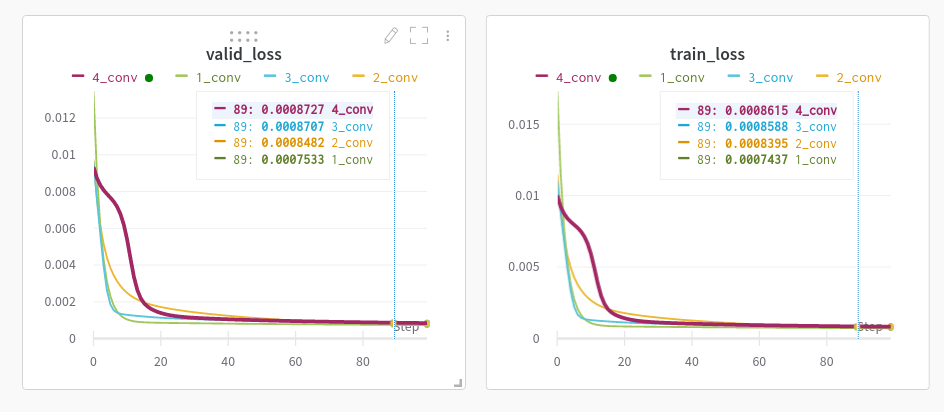
\includegraphics[width=0.75\textwidth]{figures/conv_layers.png}
        \caption{Effect of Different Conv Layers}
        \label{fig:conv_layers}
    \end{figure}

    \begin{figure}[!htb]
        \centering
        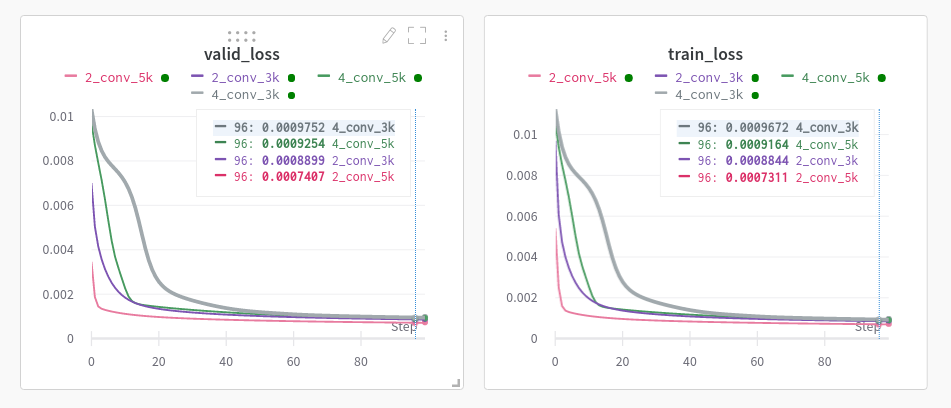
\includegraphics[width=0.75\textwidth]{figures/conv_kernels.png}
        \caption{Effect of Different Kernel Sizes}
        \label{fig:conv_kernels}
    \end{figure}

    \begin{figure}[!htb]
        \centering
        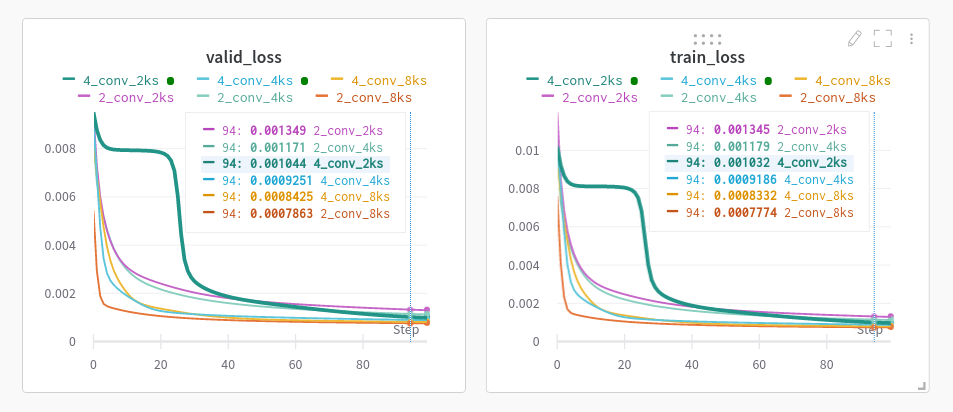
\includegraphics[width=0.75\textwidth]{figures/conv_num_kernels.png}
        \caption{Effect of Different Number of Kernels}
        \label{fig:conv_num_kernels}
    \end{figure}

    \begin{figure}[!htb]
        \centering
        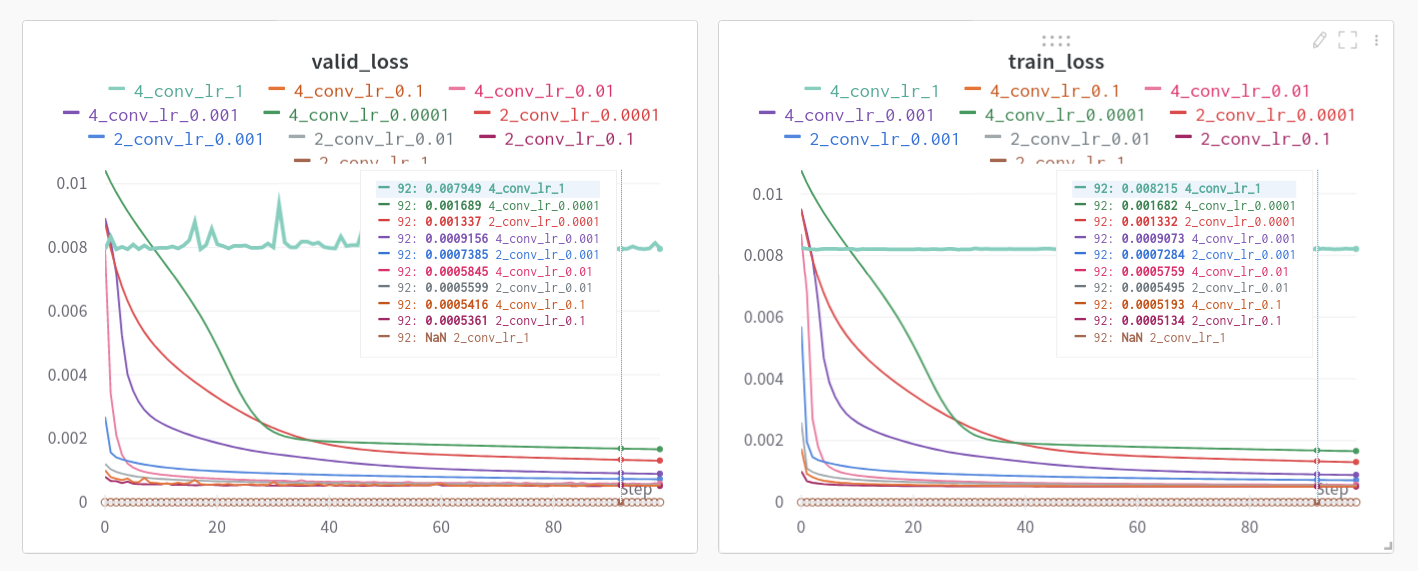
\includegraphics[width=0.75\textwidth]{figures/learning_rate/conv_lr.png}
        \caption{Effect of Different Learning Rates}
        \label{fig:conv_lr}
    \end{figure}



\section{Further Experiments (20 pts)}
    Based on your qualitative results (do not forget to give them),
    \begin{itemize}
        \item Try adding a batch-norm layer (torch.nn.BatchNorm2d) into each convolutional layer. How does it affect the results, and, why? Keep it if it is beneficial. 
        \item Try adding a tanh activation function after the very last convolutional layer. How does it affect the results, and, why? Keep it if it is beneficial. 
        
        \item Try setting the number of channels parameter to 16. How does it affect the results, and, why? Keep it if it is beneficial. 
        
      
    \end{itemize}

    \vspace*{0.5cm}

    \begin{center}
        \raggedright
        I compared my results with respect to two baselines for different number of convolutional layers, 4-conv and 2-conv.
        Overall, my observations are aligned for both 2-conv and 4-conv. All of the experiments in this part are summarized in Figure-\ref*{fig:part-2} with following abbreviations; bn: batch-norm experiment, tanh: tanh experiment, c16: 16 channel experiment. 2-conv and 4-conv stands for 2 and 4 conv layer NN respectively.
        \\
        Common Hyperparameter Baseline in Exp: \\
        learning-rate = 0.1, batch-size = 16, epoch = 100, kernel-size=5
        \\~\\

        Usually, batch-norm increases the performance of NN since scaling eases optimization during learning.
        However, BatchNorm2d increased mse loss for both 2-conv and 4-conv, its loss is the highest among all observations in Figure-\ref*{fig:part-2}.
        The reason might be because, the input and ouput data are already scaled to the interval of [-1,1], so model doesn't have any benefit in this configuration.
        However, it has some regularization effect on the weights and as a result it requires more data for training and increases the loss.
        Therefore, I don't see much of a benefit for batch-norm and I'm not planning to keep it under this configuration.
        \\~\\

        I've expected tanh to improve the model's accuracy and decreasing the loss. I've observed in Figure-\ref*{fig:part-2} that
        for 4-conv tanh decreases the loss as expected, however for conv-2 the behaviour is opposite, the loss is higher than 2-conv-base.
        This might be because of the fact that, when we change the network, even 1 single additional activation function yields another different optimization problem,
        hence our baseline hyperparameters eg. learning-rate might not be the optimal for that configuration.
        In addition, these loss curves correspond to avg loss per pixel and also all of these individual pixel values are scaled to the interval of [-1,1]  which is relatively small. Hence all of these models result in a very low mse loss value
        and loss differences between the models are marginal, so we need to make use of accuracy checking mechanisms like 12-margin and also manual image inspection.
        For example, I observe that applying tanh in both 2-conv and 4-conv has removed exploding pixel values eg. small blue segments in the image which is an improvement, but not directly visible in mse loss.
        Tanh works because we are squeezing our network's output to [-1,1] and our labels are also in this range. However, if we didn't apply tanh to conv output, it would be theoretically unbounded
        which could be more difficult to learn, in a way we are guiding the network to learn better since we have prior knowledge about our ground truth interval.
        Consequently, I'll keep tanh activation for the last layer. 
        \\~\\

        Number of channels or number of kernels that I've experimented with so far were 2, 4, and 8 as mentioned in the HW description.
        In this experiment, I've set channel-out=16 for all conv layers except for the last one which had to be 3 (r,g,b).
        I've expected a higher channel number to decrease the loss and this phenomenon is observable in Figure-\ref*{fig:part-2} where
        losses are the lowest among all of the models in this part for both 4-conv and 2-conv.
        Having higher number of channels/kernels gives our model more capacity to extract more different features from images
        and the model makes use of more of these features to fit the problem/data in a better way as a result decreasing the loss.
        Therefore, I'll keep channels as 16 since it improved our model by considerable amount. 


    \end{center}

    \begin{figure}[!htb]
        \centering
        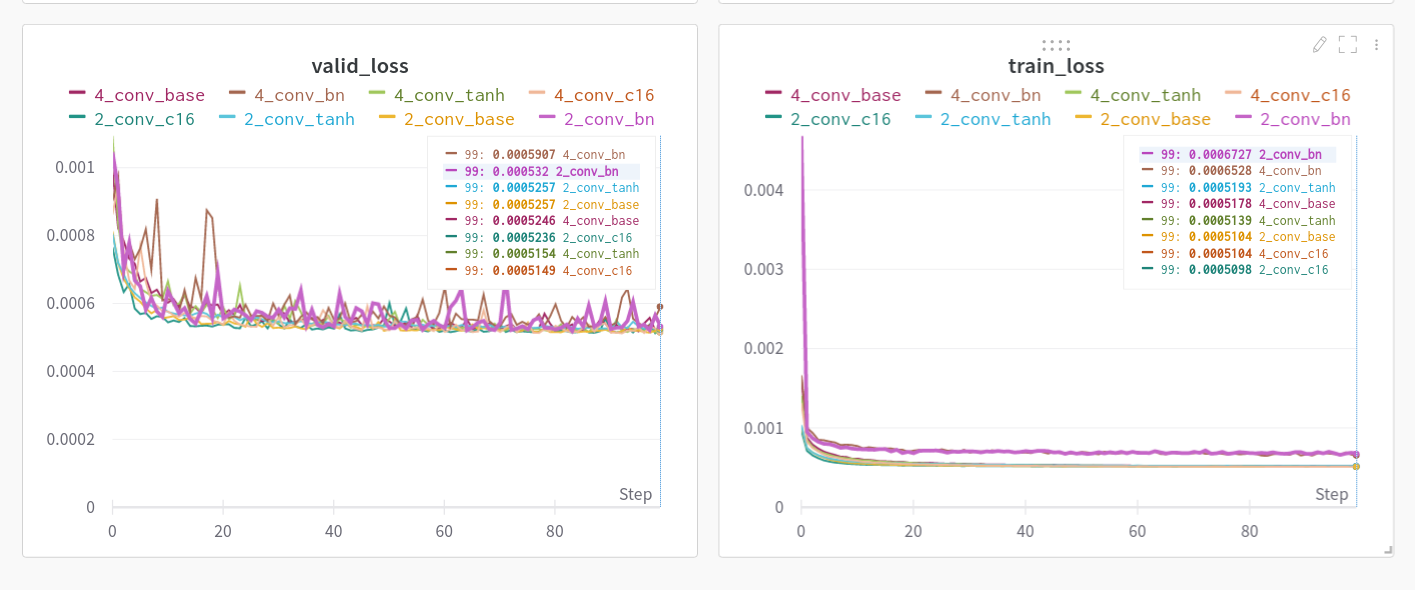
\includegraphics[width=0.75\textwidth]{figures/part-2.png}
        \caption{Effect of batch-norm, tanh, channels}
        \label{fig:part-2}
    \end{figure}

\section{Your Best Configuration (20 pts)}
Using the best model that you obtain, report the following:
 
    \begin{itemize}
        \item The automatically chosen number of epochs(what was your strategy?):
        \item The plot of the training mean-squared error loss over epochs:
        \item The  plot  of  the  validation  12-margin  error  over  epochs (see the3 text for details):
        \item At least 5 qualitative results on the validation set, showing the prediction and the target colored image:
        \item Discuss the advantages and disadvantages of the model, based on your qualitative results, and, briefly discuss potential ways to improve the model:
    \end{itemize}

    \begin{center}
        \raggedright
        Best model I've obtained so far has the following hyperparameter configuration:
        \\
        learning-rate=0.1, kernel-size=5, kernel-num=16, out-activ=tanh, conv-layers=2
        \\~\\
        For automatically choosing the number of epochs, I've monitored training with validation loss values. Namely,
        I've compared previous epoch's validation loss to the current epoch's validation loss and
        if we don't have sufficient improvement more than epsilon or if our model's loss increases more than epsilon
        for more than patience number of times then we stop learning and take our model's configuration at the epoch of (current epoch - patience) where
        patience determines the amount of toleration and epsilon is the small difference value that determines whether change should be considered as success or not.
        I've set epsilon = 5e-6  and patience = 5. The learning has stopped at 47 th epoch which is determined by our mechanism automatically.
        \\~\\
        The plot of both training and validation MSE Loss over epochs is illustrated in Figure-\ref*{fig:part-3_best_config_mse_loss} below.
        \\~\\
        The plot of both training and validation 12-Margin Loss over epochs is illustrated in Figure-\ref*{fig:part-3_best_config_12margin_loss} below.

    \end{center}

    \begin{figure}[!htb]
        \centering
        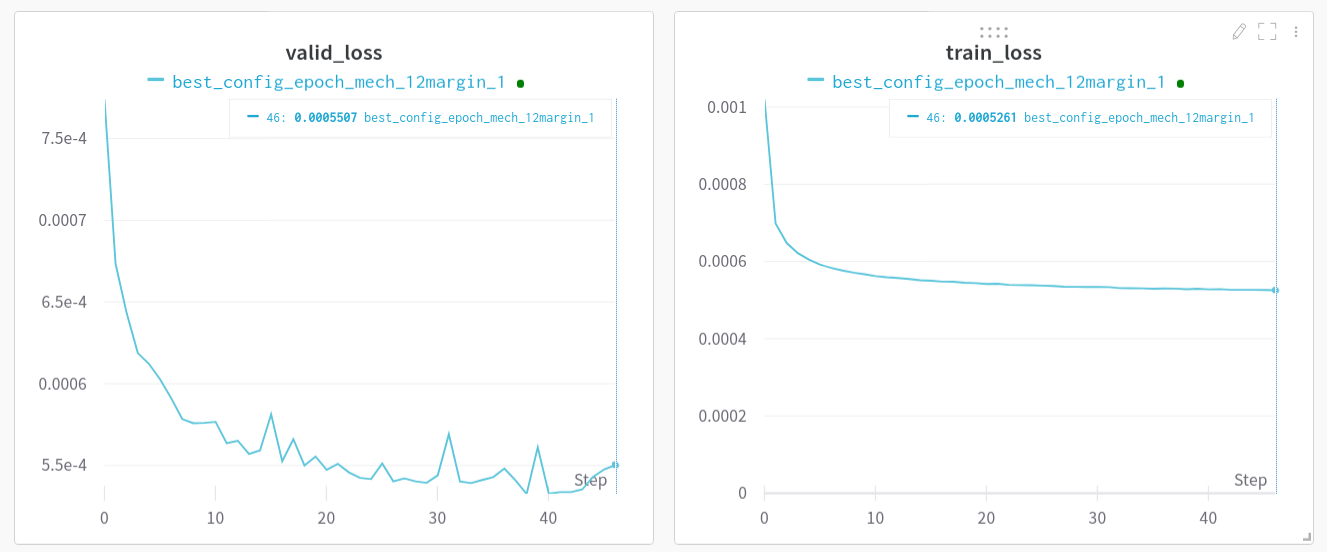
\includegraphics[width=0.75\textwidth]{figures/best_config_loss_mse.png}
        \caption{MSE Loss Curves for best configuration}
        \label{fig:part-3_best_config_mse_loss}
    \end{figure}
    
    \begin{figure}[!htb]
        \centering
        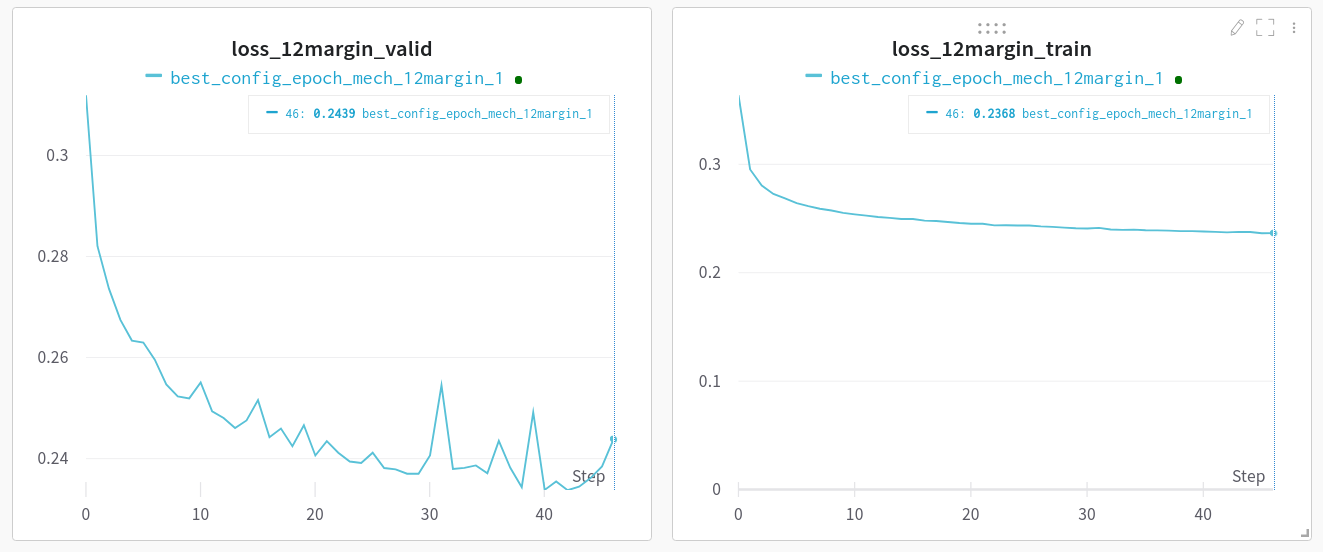
\includegraphics[width=0.75\textwidth]{figures/best_config_loss_12margin.png}
        \caption{12-Margin Loss Curves for best configuration}
        \label{fig:part-3_best_config_12margin_loss}
    \end{figure}

\section{Your Results on the Test Set(30 pts)}
This part will be obtained by us using the estimations you will provide. Please tell us how should we run your code in case of a problem:

\section{Additional Comments and References}

Throughout this assignment and experiments, I've made use of wandb for data visualization and logging.
All of my experiments are logged and can be monitored. In case any further inspection is needed check out the following wandb experiment report at url:
----<!!>----





\end{document}

